\documentclass[letterpaper, 10pt]{report}
\title{Clemson Hack Pack}
\author{Clemson ACM}
\date{\today}

\usepackage{makeidx}
\usepackage{multicol}
\usepackage{geometry}
\usepackage{tabularx}
\usepackage{pdfpages}
\geometry{margin=1in}

% Pad out huge chapter numbers in the TOC
\usepackage{tocloft}

% Custom command for inline code.
\newcommand{\code}[1]{\texttt{#1}}

% Paragraph spacing should be easy!
\usepackage{parskip}

% Chapter title format: "X. Chaptertitle", not "Chapter X\nChaptertitle".
% Also, make \sections stand out a bit more.
\usepackage{titlesec}
\titleformat{\chapter}[block]{\normalfont\huge\bfseries}{\thechapter.}{1em}{\Huge}
\titleformat{\section}[block]{\normalfont\large\bfseries}{\thesection.}{1em}{\LARGE}

% Adjust spacing around headers to reduce empty space
\titlespacing*{\chapter}{0pt}{-22pt}{-1pt}
\titlespacing*{\section}{0pt}{10pt}{0pt}
\titlespacing*{\subsection}{0pt}{10pt}{0pt}
\titlespacing*{\subsubsection}{0pt}{0pt}{0pt}

% Citations should use superscript. It's nice.
\usepackage[superscript, biblabel]{cite}

% Use the Bera font family (based on Bitstream Vera) for text (bera), captions
% (berasans), and code (beramono).
\usepackage{bera}
\usepackage[scaled]{berasans}
\usepackage[scaled]{beramono}
\usepackage[T1]{fontenc}

% Needed for the inclusion of graphics.
\usepackage{graphicx}

% Allows the use of EPS files, a type of vector graphic.
\usepackage{epstopdf}

% Use the listings package for pretty source code inclusions.
\usepackage{color}
\usepackage{xcolor}
\usepackage{soul}
\usepackage{listings}
\lstset{
  basicstyle=\footnotesize\ttfamily, % Use a truetype, footnote-sized font.
  numbers=left,                      % line numbers go on the left
  numbersep=10pt,                    % how far the line-numbers are from the code
  tabsize=2,                         % sets default tabsize to 2 spaces
  extendedchars=true,                % lets you use non-ASCII characters; for 8-bits encodings only
  breaklines=true,                   % sets automatic line breaking
  keywordstyle=\bfseries,            % Keyword styling
  numberstyle=\ttfamily\color{gray}, % the style that is used for the line-numbers
  stringstyle=\color{gray},          % string literal style
  commentstyle=\itshape\color{gray}, % comment literal style
  title=\lstname,                    % show the filename of files included with \lstinputlisting
  frame=b,                           % show a frame along the bottom
  rulecolor=\color{lightgray},
  language=C++,                      % the default language of the code
  showspaces=false,                  % show spaces as space, not a litle underscore.
  showstringspaces=false             % same as above, in strings.
  showtabs=false,                    % same as above, with tabs.
  xleftmargin=17pt,
  framexleftmargin=17pt,
  framexrightmargin=5pt
}

% Listings caption configuration.
\usepackage{caption}
\DeclareCaptionFont{white}{\color{white}}
\DeclareCaptionFormat{listing}{\colorbox[cmyk]{0.43, 0.35, 0.35,0.01}{\parbox{\textwidth}{\vspace{1.5pt}\hspace{10pt}#1#2#3}}}
\captionsetup[lstlisting]{format=listing,labelfont=white,textfont=white, singlelinecheck=false, margin=0pt, font={bf, sf}}

% Defines a tikz frame for page-broken listing hints.
% Shamelessly stolen from https://tex.stackexchange.com/questions/77996/how-to-show-a-hint-when-lstlisting-is-breaking-page
\usepackage[framemethod=tikz]{./formatting/mdframed}
\mdfdefinestyle{note}
  {
    hidealllines = true ,
    skipabove    = .5\baselineskip ,
    skipbelow    = .5\baselineskip ,
    singleextra  = {} ,
    firstextra   = {
      \node[right,overlay,align=center,font=\continuingfont]
        at (O) {\continuingtext};
    } ,
    secondextra  = {
      \node[above right,overlay,align=left,font=\continuingfont]
        at (O |- P) {\continuedtext};
    } ,
    middleextra  = {
      \node[right,overlay,align=left,font=\continuingfont]
        at (O) {\continuingtext};
      \node[above right,overlay,align=left,font=\continuingfont]
        at (O |- P) {\continuedtext};
    }
  }

% Sets up the hint content and style for page-broken listings.
\newcommand*\continuingfont{\color{gray}\footnotesize\itshape}
\newcommand*\continuingtext{Continues on next page}
\newcommand*\continuedtext{Continued from previous page}

% A wrapper command for automatically wrapping input listings
% with a hintable frame.
\newcommand{\acmlisting}[2][]
{
\mdframed[style=note]
\lstinputlisting[#1]{#2}
\endmdframed
}

% Turn on the powerful indexing features
\makeindex

% Make links, footnotes, etc. clickable, and generate pdf bookmarks.
\usepackage{hyperref}
\hypersetup{
  pdfauthor={Clemson ACM, acm@cs.clemson.edu},
  pdfcreator={Clemson ACM, acm@cs.clemson.edu},
  pdftitle={Clemson ACM Hack Pack},
  pdfsubject={Clemson ACM Hack Pack},
  unicode=true,
  colorlinks=false,
  pdfborder=0 0 0,
  bookmarks=true
}



\begin{document}
\maketitle

\section*{Copyright}
The content of all `.tex' files is available under the GFDL. \\
Copyright (C)  2015  Clemson ACM \\
Permission is granted to copy, distribute and/or modify this document
under the terms of the GNU Free Documentation License, Version 1.3
or any later version published by the Free Software Foundation;
with no Invariant Sections, no Front-Cover Texts, and no Back-Cover Texts.
A copy of the license is included in the section entitled "GNU
Free Documentation License".\\

The content of all other files is available under the GPLv3. \\
The Hackpack is a concise and extensive cheatsheet/guide designed to be used during ACM-style programming competitions. \\
Copyright (C)  2015  Clemson ACM \\

This program is free software: you can redistribute it and/or modify
it under the terms of the GNU General Public License as published by
the Free Software Foundation, either version 3 of the License, or
(at your option) any later version.

This program is distributed in the hope that it will be useful,
but WITHOUT ANY WARRANTY; without even the implied warranty of
MERCHANTABILITY or FITNESS FOR A PARTICULAR PURPOSE\@. See the
GNU General Public License for more details. \\

You should have received a copy of the GNU General Public License
along with this program. If not, see <http://www.gnu.org/licenses/>.


\break

\input{./general/tencommandments.tex}

\tableofcontents

\chapter{Data Structures}
\input{./structures/set/set}
\input{./structures/map/map}
\section{Heap}\index{heap}\index{priority\_queue}
Heaps are very useful data structures that support at least the following operations:


\begin{itemize}
	\item Insert
	\item Either:
		\begin{itemize}
			\item Remove the smallest element 
			\item Remove the largest element
		\end{itemize}
\end{itemize}

Heaps that support removing the smallest element are called ``Min Heaps''
Heaps that support removing the largest element are called ``Max Heaps''
Many other implementations also implement a decrease key operation and delete operation.

The standard template library provides a two sets of functions that provide heaps.
By default, both implementations are ``Max Heaps'' but can be made to be ``Min Heaps''.
The first is the \lstinline{priority_queue} data structure found in the queue header.
The second is the \lstinline{make_heap} functions in found the algorithm header.
Neither of these implementations strictly implements the decrease key operation.
The code sample shown below shows how to create a Binary Min Heap as well in $O(N)$ time as the Heap Sort algorithm which runs in $O(N \log N)$ time.

\subsection{Reference}
\acmlisting[caption=Heap Reference, label=Heap Reference]{./structures/heap/heap.cpp}

\subsection{Applications}
\begin{itemize}
	\item Dijkstra's Algorithm
	\item Prim's Algorithm
	\item Priority Based Queuing
\end{itemize}

\section{Graph}
Graphs are useful for a variety of different real world problems.
Graphs are comprised of Nodes and Edges.
Nodes represent a distinct state.
Edges represent the possible transitions between states.
Graphs can be directed(edges are one way) or undirected(edges are the same going to or from a node).

Paths are graphs that have no branches off.
Cycles are graphs that connect back on them selves.
Trees are graphs that contain no cycles.
Forests are graphs that contain multiple disjoint trees.
Bipartite Graphs have a set of "source" nodes and a set of "edge" nodes

Two nodes $i,j$ are said to be connected if there is a path from i to j.
Two nodes $i,j$ are said to be strongly connected if there is a directed path from i to j and j to i.

\subsection{Reference}
\acmlisting[caption= Undirected Graph, label=Undirected Graph]{./structures/graph/graph.cpp}

\subsection{Applications}
For all run times, $V$ is the number of nodes, and $E$ is the number of edges.
\begin{itemize}
	\item Shortest Paths
		\begin{itemize}
			\item Breath First Search --- Graphs with equal weight edges $O(V+E)$
			\item Dijkstra's Algorithm --- Graphs with non-negative edges weights $O(E \log V)$.
			\item Bellman Ford --- Graphs with some negative edges $O(VE)$
			\item Floyd Warshall --- Graphs with negative edges but not cycles $O(V^3)$.
			\item Dynamic Programming --- Directed Acyclic Graphs various running times.
		\end{itemize}
	\item Minimum Spanning Trees 
		\begin{itemize}
			\item Prim's Algorithm --- For undirected graphs; if run for each component, finds the minimum spanning forest$O(E \log V)$.
			\item Kruskal's Algorithm --- For graphs; finds the minimum spanning forests in unconnected graphs $(E \log V)$
		\end{itemize}
	\item Similarity/Connectivity
		\begin{itemize}
			\item Depth First Search --- Find (Strongly) Connected Components $O(V+E)$
			\item Depth First Search --- Find a path from i to j $O(V+E)$
		\end{itemize}
	\item Topological Sorting 
		\begin{itemize}
			\item Depth First Search --- Use start and stop times to topologically sort $O(V+E)$
		\end{itemize}
	\item Matchings
		\begin{itemize}
			\item Greedy --- Many of these problems can be solved by a greedy max/min flow algorithm in $O(EV \log V \log F)$ where F is is the max flow.
		\end{itemize}
	\item Flow/Routing
		\begin{itemize}
			\item Greedy --- Many of these problems can be solved by a greedy max/min flow algorithm in $O(EV \log V \log F)$ where F is is the max flow.
		\end{itemize}
	\item Clustering
	\item Centrality
\end{itemize}

#ifdef hackpackpp
\subsection{Sample Contest Problem, The Cows Escape}
Farmer John's Farm has become infested with Zombies!
Farmer John being slightly out of shape wants to take the shortest amount of time to escape the zombies.

Farmer John's Farm is laid out in squares.
Being prepared, Farmer John has his Early Zombie Detection System that will alert him to the rating of the zombies in these squares.
Based off his research into the topic, Farmer John knows based on the rating how long it will take to evade the zombies in that sector.

Help Farmer John find the shortest time it will take Farmer John to escape his farm with his cows.

\subsubsection{Input Format}
\begin{itemize}
	\item Line 1:One integer $T$ indicating the number of test cases to evaluate
	\item Line 2:Three integers $k,w,h$ representing the number zombie classes to follow and the width and height of Farmer John's Farm
	\item Lines 3..$(3+k)$: The letter representing the zombie class, it will not be `F' and the time it will take to evade them, $t$
	\item Lines $(4+k)$..$(4+k+h)$: $W$ capital letters representing the zombie classes in each sector of farmer John's farm.  Farmer John's initial position is designated by `F'.
\end{itemize}

\subsubsection{Sample Input}
\acmlisting[caption=The Cows Escape Sample Input, label= The Cows Escape Sample Input]{./structures/graph/problems/escape/escape.in}

\subsubsection{Output Format}
\begin{itemize}
	\item Line 1:  1 integer per line for each test case representing the minimum time it takes to escape the farm.
\end{itemize}

\subsubsection{Sample Output}
\acmlisting[caption=The Cows Escape Sample Output, label= The Cows Escape Sample Output]{./structures/graph/problems/escape/escape.out}
\subsubsection{Sample Solution}
#endif

#ifdef hackpack
\subsection{Dijkstra in a graph}
#endif
\acmlisting[caption=The Cows Escape Sample Solution, label= The Cows Escape Sample Solution]{./structures/graph/problems/escape/escape.cpp}

#ifdef hackpackpp
\subsubsection{Lessons Learned}
\begin{itemize}
	\item Dijkstra can be solved using a priority queue using $O(N \log N)$ time.
\end{itemize}
#endif


\section{Segment Tree}
\index{segment tree}
\index{interval}

% #ifdef hackpackpp

It is often useful to be aware of the range properties of a given array, such as: prefix sums, suffix sums, range minimum queries, range maximum queries, etc.
For simpler problems, a secondary array may suffice to calculate a property like the prefix sum of an array.
The prefix sum calculation only takes $O(n)$ time to perform, and any query thereafter takes only $O(1)$ time.
But any updates to the source dataset will require $O(n)$ time to update the prefix sum calculations.
Frequent changes will quickly show the pitfall of this approach.
A segment tree is a data structure for storing information about intervals that can be constructed in $O(n)$ time.
Whenever the source data changes, update times stay low at $O(\log n)$ time.

% #endif

% #ifdef hackpack

A segment tree is represented as an array of a size that is dependent on the dataset it is sourced from.
For a given array of size $n$, a segment tree constructed from it will use up to $2^{\lceil \log_2 (n)\rceil + 1} - 1$ space.
Once built, the structure of a segment tree cannot change.

% #endif

% #ifdef hackpackpp

\begin{figure}[h]
    \centering
    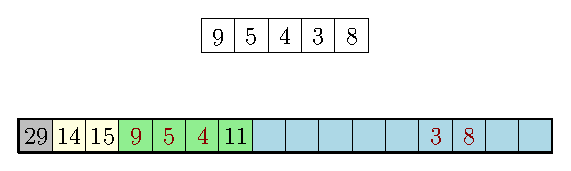
\includegraphics[width=0.6\textwidth]{./structures/segment-tree/source-array}
    \caption{\small The segment tree (bottom) constructed from an array (top) containing five elements.
      The blank entries in the segment tree array are unused.}
\end{figure}

A segment tree is represented as an array of a size that is dependent on the dataset it is sourced from.
For a given array of size $n$, a segment tree constructed from it will use up to $2^{\lceil \log_2 (n)\rceil + 1} - 1$ space.
To properly represent tree, the root is located at index 0; its left and right children are located at indices 1 and 2 respectively.
To properly recurse through the tree, indices of left and right children can be calculated with $2n + 1$ and $2n + 2$ for left and right children respectively.

Construction of a segment tree begins at the root.
The root node, located at index 0, queries its two children for some property (such as the maximum, the minimum, a range sum, etc\ldots).
Those two children, in turn, query their children.
This process continues until a leaf node, one of the values from the source array, is reached.
The recursive calls return back up the call stack with the parent nodes receiving the information they requested.
These parent nodes record this information and continue returning up the call stack.

As the recursive calls are made, the starting and ending indices that each node represents is passed on.
The left child of a node represents the first half of the section of the dataset the parent represents.
The right child of a node represents the remaining right half.
More precisely, if the parent node represents values between and including a starting index, $a$, and ending index $b$, then the left child will represent values between and including $a$ and $a + \frac{b - a}{2}$.
The right child will represent values between and including $a + \frac{b - a}{2} + 1$ and $b$.
When $a$ and $b$ are equal, a leaf node has been reached, and its value is simply stored at the appropriate index in the segment tree.
Due to the static nature of arrays, once built, the structure of a segment tree cannot change.

\begin{figure}[h]
    \centering
    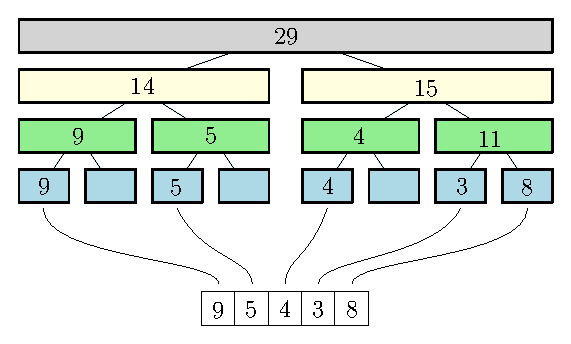
\includegraphics[width=0.6\textwidth]{./structures/segment-tree/array-tree}
    \caption{\small The segment tree visualized in a tree-like format.
    The leaves of the tree are values from the original dataset.}
\end{figure}

% #endif

% #ifdef hackpack

\acmlisting[label=Segment Tree Reference Code, caption=Segment Tree Reference Code]{./structures/segment-tree/segment-tree.cpp}

% #endif


% #ifdef hackpackpp

Generally, a segment tree supports two operations: update and query.
The update operation will account for changes to values in the source dataset.
It is even possible to implement a range update operation to change an entire range of values.
The query operation allows for fast retrieval of segment information.
In the case of the prefix sum, the update operation will modify the tree's nodes such that it will contain correct information after changes, and the the query operation can return a sum for values in an arbitrary range.

\subsection{Applications}

\begin{itemize}
    \item range sums in a frequently changing dataset
    \item range minimum/maximum queries
\end{itemize}

\subsection{Example Contest Problem: Coming and Going}

Farmer John is considering expanding the cows' barn, but he would first like to learn just how many of his cows spend any given time of day in the barn.
In consideration of expanding the cows' barn, Farmer John decided to see just how many of his cows spent any given time of day in the barn.
To do so, he installed motion sensors on each entryway/exit to the building.
These sensors are able to detect both the entry and exit of a warm-blooded being.
This, coupled with his cows' tags, allows him to monitor the movements of specific cows.

The night after the full day in which the sensors were installed, Farmer John sat down to do what he thought was some straightforward analysis, but quickly realized that he was in over his head with only mental math.
He dusts off his old Commodore 64 and begins tabulating the data that he has collected.
Among this data are the times that individual cows were inside the barn.
\textit{While} he enters these times into the computer for each cow, Farmer John wants to see how many cows were inside the barn during a specific time range.

Help him figure out how many cows were inside the barn during specific time ranges as he (slowly) tabulates the data.

\subsubsection{Input Format}

\begin{itemize}
    \item Line 2: A single integer, $C$, representing the number of cows Farmer John has data on.

    \item The following lines are placed in $C$ groups detailed as follows:
    \begin{itemize}
        \item A single line containing a single integer, $k$, representing the number of time ranges to follow that the cow was present in the barn.

        \item $k$ lines with two distinct integers representing times between which a cow was present in the barn.
        The first number is guaranteed to be strictly less than the second number.
        \item A single line containing two integers $t_1$ and $t_2$ representing times between which the maximum number of cows seen in the barn simultaneously should be reported since the last cow's data was added.
        As usual, with time ranges, the range $t_1$ to $t_2$ includes $t_1$ and all hours leading up to, but excluding $t_2$.
    \end{itemize}
\end{itemize}

\acmlisting[label=Coming and Going Sample Input, caption=Coming and Going Sample Input]{./structures/segment-tree/problems/coming-and-going/coming-and-going.in}

\subsubsection{Output Format}

$C$ lines indicating the maximum number of cows seen in the barn in a single hour after adding data for the 1\textsuperscript{st}, 2\textsuperscript{nd}, \ldots, $C$\textsuperscript{th} cow.
Each should appear on its own separate line formatted as given in the sample output.

\acmlisting[label=Coming and Going Sample Output, caption=Coming and Going Sample Output]{./structures/segment-tree/problems/coming-and-going/coming-and-going.out}

\subsubsection{Sample Solution}

% #endif

\acmlisting[label=Coming and Going Sample Solution, caption=Coming and Going Sample Solution]{./structures/segment-tree/problems/coming-and-going/coming-and-going.cpp}

% #ifdef hackpackpp

\subsubsection{Lessons Learned}

\begin{itemize}
    \item The data the segment tree keeps track of can easily be changed with a few small modifications to the build, update, and query operations.
\end{itemize}

% #endif


\chapter{Algorithms}
\input{./algorithms/dijkstra/dijkstra}
\input{./algorithms/sieve-of-eratosthenes/sieve-of-eratosthenes}
\input{./algorithms/kmp-string-matching/kmp-string-matching}
\input{./algorithms/computational-geometry/comp-geom}
\section{Flood Fill}
\index{flood fill}

This is an algorithm that will, given some starting node(s), proceed to explore an entire graph by 'spreading' in all directions, hence, its name.
A sort of boundary can also be applied to limit the extent of 'flooding' the algorithm does.
More specifically, it can be used to 'color' or mark nodes in a certain manner.
It can be seen as a more specific example of breadth- or depth-first search.
A flood fill can be implemented with either a queue or a stack and runs in $O(n)$ time.

\begin{figure}[h]
    \centering
    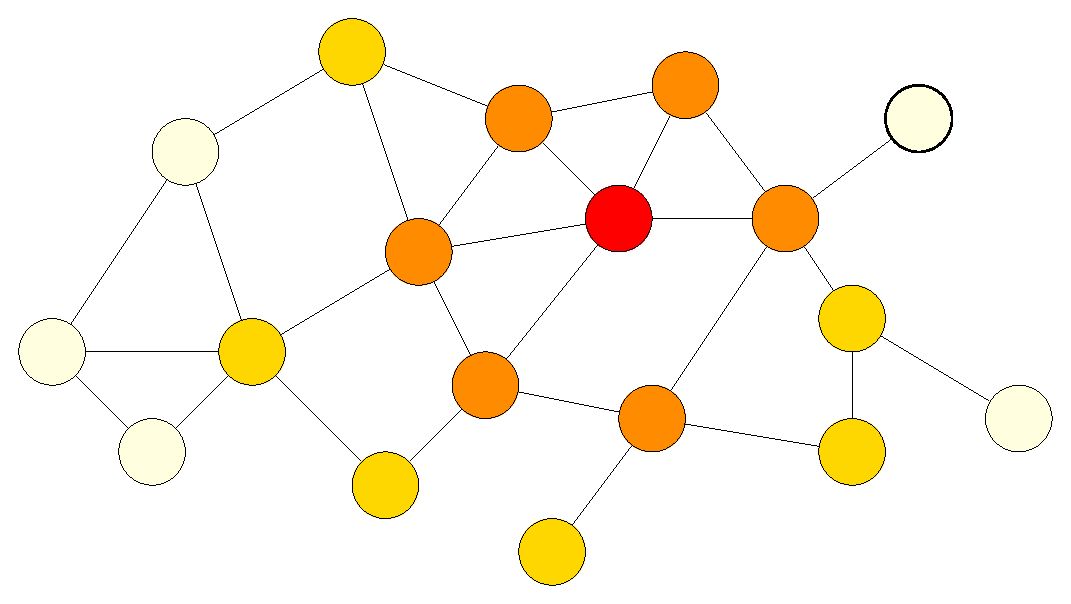
\includegraphics[width=0.6\textwidth]{./algorithms/flood-fill/partial-ff}
    \caption{\small A complete flood fill on a graph.
      The red node is where the algorithm started.
      Nodes visited later in the algorithm are progressively more yellow.}
\end{figure}

\input{./algorithms/breadth-first-search/breadth-first-search}
\input{./algorithms/depth-first-search/depth-first-search}
\section{Prim's Algorithm}\index{graph!Prim's Algorithm}
#ifdef hackpackpp
Prim's algorithm is a greedy algorithm that allows for finding a minimum spanning tree/forest in $O(E  \log{V})$ time.
Prim's algorithm is implemented by doing the following:

\begin{enumerate}
	\item Choose an arbitrary unvisited node in the graph.
	\item Grow the tree by choosing the node that can be added to the tree by least cost.
	\item Repeat step 2 until all connected nodes have been visited. If there are still nodes, return to step 1.
\end{enumerate}

#endif
\subsection{Applications}
\begin{itemize}
	\item Finding a minimum spanning tree
\end{itemize}

#ifdef hackpackpp
\subsection{Example Contest Problem: Cow Connection}
Farmer John has expanded his real estate holdings and now owns several farms.
These farms are connected by an old, unmaintained road network. 

At night, these roads are unlit and are very dangerous.
Farmer John wants to improve safety by installing lights along the roads.
However, Farmer John does not have much extra money to spend on this effort.

Help Farmer John determine a minimum cost set of roads that he could light to connect all of the farms by lit roads.
\subsubsection{Input Format}
\begin{itemize}
\item Line 1: One integer, $N$, $(N < 1000000)$ specifying the number of paths in the corn field.
\item Line 2..$(N+1)$: Each line contains three integers $S$, $D$ and $C$ where:
	\begin{itemize}
		\item $S$ and $D$ represent the farm id numbers that a given road connects. $0 \leq S < N$ and $0 \leq D < N$.
		\item $C$ is the cost of lighting that road. $(0 < C < 1000000$
	\end{itemize}
\end{itemize}

\subsubsection{Sample Input}
\acmlisting[label=Cowconnection Sample Input, caption=Cowconnection Sample Input]{./algorithms/prims-algorithm/problems/cowconnection/cowconnection.in}
\subsubsection{Output Format}
\begin{itemize}
	\item Line 1: One integer, representing the minimum cost.
	\item Line 2..$(N+1)$: Two integers, that represent the farms at the end of either road Farmer John should choose to light.
		These integers should be in order from least to greatest.
\end{itemize}
\subsubsection{Sample Output}
\acmlisting[label=Cowconnection Sample Output, caption=Cowconnection Sample Output]{./algorithms/prims-algorithm/problems/cowconnection/cowconnection.out}
\subsubsection{Example Solution}
#endif

#ifdef hackpack
\subsection{Prim's Algorithm}
#endif
\acmlisting[label=Cowconnection Example Solution, caption=Cowconnection Example Solution]{./algorithms/prims-algorithm/problems/cowconnection/cowconnection.cpp}
#ifdef hackpack
\subsubsection{Lessons Learned}
\begin{itemize}
	\item Typedefs can greatly improve readability of code
	\item Convenience classes can greatly improve readability
	\item Directed graphs can be converted to undirected graphs by inserting the edge for both the source and the destination.
\end{itemize}
#endif


\section{Max Flows}\index{graph!Max Flows}
#ifdef hackpackpp
This section does not attempt to define basic terms regarding graphs.
For these definitions, please review the section entitled graphs in the data structures section of the hackpack.


There are several types of problems that involve finding maximum flow in a graph.
Many of these problems can easily tackled by making small transformations to the graph.


The implementation below solves the max flow problem for a single source and sink.
If there is more than one source or sink, one can add a ``super'' source and or sink that connects to all of the sources and sinks.
Then find the flow from the super source to the super sink.


The implementation below solves the maximum flow problem for directed graphs.
If the graph is undirected, simply insert every edge twice in both directions.


The implementation below places the weights on the edges instead of the nodes.
If the flow is limited through the nodes instead of the edges, simply split every node into an ``in'' node and an ``out'' node and place the weight on the path between them.


In a general directed graph, this can be done in $O(EV \log V \log F)$ where E is the number of edges V is the numbr of nodes, and time where F is the maximum flow.
\begin{itemize}
	\item While there is a path from source to sink
	\begin{itemize}
		\item Greedily find the widest path --- the single path with greatest capacity.
		\item Reduce the capacity of the edges on the widest path by the capacity of the widest path.
		\item Increase the capacity of the edges on the widest path by the capacity of the widest path going in the opposite direction creating them if necessary.
	\end{itemize}
\end{itemize}

#endif

\subsection{Applications}
\begin{itemize}
	\item Finding the maximum flow in a graph
	\item Finding a minimum set of edges required to disconnect source and sink
	\item Finding a maximal matching
\end{itemize}
#ifdef hackpackpp

\subsection{Example Contest Problem: Cow-Ex}
The cows have opened up a package distribution system.

The cows have several routes by which they distribute packages.
Each route has been rated with a positive integer referring to the amount of packages that the route can carry in 1 day.

Today is Farmer John's birthday, and the cows wish to send him as many packages as possible.
Help the cows determine the how many packages they can send to Farm John's barn.
\subsubsection{Input Format}
\begin{itemize}
	\item Line 1: A positive integer N that represents the number of routes that the cows have in place. $0 < N \leq 10000$
	\item Line 2..$(N+1)$: Three non-negative integers, $S$, $D$, $E$ representing a route going from location $S$ to location $D$ with a capacity of $E$. $0 \leq S,D < N$
	\item Line $(N+2)$: A non-negative integer $A$, that represents location where packages are sent.
	\item Line $(N+3)$: A non-negative integer $B$, that represents location of the barn.
\end{itemize}

\subsubsection{Sample Input}
\acmlisting[label=Cowex Sample Input, caption=Cowex Sample Input]{./algorithms/max-flow/problems/cowex/cowex.in}

\subsubsection{Output Format}
\begin{itemize}
	\item Line 1: A Positive integer representing the maximum capacity of the network.
		This should be 0 if it is not possible to transport any packages.
\end{itemize}
\subsubsection{Sample Output}
\acmlisting[label=Cowex Sample Output, caption=Cowex Sample Output]{./algorithms/max-flow/problems/cowex/cowex.out}
\subsubsection{Example Solution}
#endif

#ifdef hackpack
\subsection{Greedy Max Flow Algorithm}
#endif

\acmlisting[label=Cowex Sample Solution, caption=Cowex Sample Solution]{./algorithms/max-flow/problems/cowex/cowex.cpp}
#ifdef hackpackpp
\subsubsection{Lessons Learned}
\begin{itemize}
	\item The innermost while loop is a solution to the widest most path problem that runs in $O(E \log V)$ time.
\end{itemize}
#endif



\chapter{Approaches}
\section{Hash Window Approaches}\index{hashing}\index{hash windows}
#ifdef hackpackpp
Hashing is a mapping of objects to bytes.
These bytes are often stored in Strings or numeric data types.
Normally, hash functions attempt to map each object to a \textit{unique} set of bytes.
Also a \textit{slight} change in the object should cause a \textit{large} change in the output.
When two objects map to the same set of bytes, it is referred to as a hash collision.

\subsection{Applications}
\begin{itemize}
	\item Identify substrings quickly and cleanly.
	\item Hash collisions to detect certain features of the input.
\end{itemize}

\subsection{Fine Print Returns!}
The cows have prepared another legal document for Farmer John to review.

The Cows are still championing the installation of an Olympic style swimming pool.
However, this time Farmer John only cares about how many times, `pool' appears in the text.

Help Farmer John determine how many times the text `pool' appears in the document.

\subsubsection{Input}
\begin{itemize}
	\item A stream of text terminated by an EOF representing the legal agreement
\end{itemize}

\subsubsection{Sample Input}
\acmlisting[label=Fine Print Sample Input, caption=Fine Print Sample Input]{./approaches/hashing/problems/fine-print/fine-print.in}

\subsubsection{Output}
\begin{itemize}
	\item 1 integer representing the number of references to the word pool in the text.
\end{itemize}

\subsubsection{Sample Output}
\acmlisting[label=Fine Print Sample Output, caption=Fine Print Sample Output]{./approaches/hashing/problems/fine-print/fine-print.out}

\subsubsection{Sample Solution}
#endif

#ifdef hackpack
\subsection{Hash Windows}
#endif
\acmlisting[label=Fine Print Sample Solution, caption=Fine Print Sample Solution]{./approaches/hashing/problems/fine-print/fine-print.cpp}
#ifdef hackpackpp
\subsubsection{Lessons Learned}
\begin{itemize}
	\item There is often more than one way to solve a problem, checkout the KMP string matching algorithm for another way to solve this problem.
\end{itemize}
#endif


\section{Dynamic Programming}\index{Dynamic Programming}
#ifdef hackpackpp
Dynamic Programming is a powerful tool that can be applied to several different types of algorithms.\cite{dppractice}
The basic idea is to save the results of smaller problems and use the results to solve larger problems.

\subsection{Applications}
\begin{itemize}
	\item	Improving runtimes of some other algorithms
	\item	Solving the knapsack in $O(nm)$ time
	\item	Solving the integer knapsack in $O(nm)$ time
	\item	Solving the largest increasing subsequence in $O(n \log n)$ time
	\item	Solving the maximum value sub-array problem in $O(n)$
	\item	Solving the maximum value continuous sub-array problem
\end{itemize}

\subsection{Example Contest Problem: A Knapsack Full of Fireworks}\index{Knapsack}
The cows on Farmer John's Farm are planning on putting on a fireworks show for Farmer John's birthday.

They have pooled all of their loose change, and hope to purchase a collection of fireworks that will maximize  Farmer John's amazement during the show so that he will be more likely to build them a new barn.
Each firework's label helpfully includes a "wow factor" rating explicitly for this purpose.
A high "wow factor" is more desirable than a low one.

Please help the cows determine the maximum "wow factor" they can get for their loose change.

\subsubsection{Input Format}
\begin{itemize}
	\item Line 1: One integer, $N$ $(1 \leq N \leq 100)$, the number of fireworks in the catalog.
   \item Line 2: One integer, $C$ $(1 \leq C \leq 10000)$, the total amount of change that the cows have to spend.
	\item Lines 3..$(N+2)$ Two integers $P,W$ representing the price and wow factor for the fireworks.
\end{itemize}

\subsubsection{Sample Input}
\acmlisting[caption=A Knapsack Full of Fireworks Input, label=A Knapsack Full of Fireworks Input]{./approaches/dp/problems/knapsack/knapsack.in}

\subsubsection{Output Format}
\begin{itemize}
	\item Line 1: A single integer representing the maximum wow factor.
\end{itemize}
\subsubsection{Sample Output}
\acmlisting[caption=A Knapsack Full of Fireworks Output, label=A Knapsack Full of Fireworks Output]{./approaches/dp/problems/knapsack/knapsack.out}

\subsubsection{Example Solution}
#endif

#ifdef hackpack
\subsection{Knapsack Problem}
#endif
\acmlisting[caption=A Knapsack Full of Fireworks Solution, label=A Knapsack Full of Fireworks Solution]{./approaches/dp/problems/knapsack/knapsack.cpp}
#ifdef hackpackpp

\subsubsection{Lessons Learned}
The optimal solution is of the form:
$$W(j) = \max \left\{W(j-1), \max \left\{W(j - p_i) + v_i \right\}\right\}$$
Where $W(0) = 0$

\subsection{Example Contest Problem: A Few Fireworks More}\index{Knapsack!Integer}
The cows have reconsidered their original plan of buying just the fireworks with the greatest total "wow factor".
Instead, they want to incorporate "wow factor" \emph{and} diversity, so the cows have decided to purchase a collection of fireworks that optimizes "wow factor" and includes no more than one of each kind of firework in the catalog.

Please help the cows determine the maximum "wow factor" they can get for their loose change, on the condition that they purchase no more than one of each kind of firework in the catalog.

\subsubsection{Input}
\begin{itemize}
	\item Line 1: One integer, $N$, $(1 \leq N \leq 100)$ the number of fireworks in the catalog.
	\item Line 2: One integer, $C$, $(1 \leq C \leq 10000)$ the number of cents that the cows found.
	\item Lines 3..$(N+2)$ Two integers $P,W$ representing the price and wow factor for the fireworks.
\end{itemize}

\subsubsection{Sample Input}
\acmlisting[caption=A Few Fireworks More Input, label=A Few Fireworks More Input]{./approaches/dp/problems/one-zero/one-zero.in}

\subsubsection{Output Format}
\begin{itemize}
	\item Line 1: A single integer representing the maximum wow factor using each firework at most once
\end{itemize}
\subsubsection{Sample Output}
\acmlisting[caption=A Few Fireworks More Output, label=A Few Fireworks More Output]{./approaches/dp/problems/one-zero/one-zero.out}

\subsubsection{Example Solution}
#endif

#ifdef hackpack
\subsection{Knapsack Problem}
#endif
\acmlisting[caption=A Few Fireworks More Solution, label=A Few Fireworks More Solution]{./approaches/dp/problems/one-zero/one-zero.cpp}
#ifdef hackpackpp

\subsubsection{Lesson Learned}
A similar problem to the knapsack, except each item can be used at most once.  The solution here is to expand the state space.  The optimal solution is of the form
$$M(i,j) = \max \left\{ M(i-1, j) , M(i-1, j- s_i) + v_i \right\}$$
Where $M(0,j) = 0$ and $M(i,0) = 0$

\subsection{Example Contest Problem: The Good, the Bad, the Cowy}\index{Largest Increasing Subsequence}
Farmer John's birthday party went off without a hitch, but the cows are worried that Farmer John isn't yet convinced that he should build the cows a new barn. Just in case, they have decided to put it to a vote whether or not they should bake him a cake as well.
Unfortunately, the cows are all experts in the school of bovine politics, and think that a simple majority vote will simply not do because of the dangers of vote rigging.

Instead, the cows have resorted to a rather odd voting system: each cow votes in some arbitrary order with an integer value, and if the length of largest increasing subsequence of all the votes is greater than half the number of cows, then the cows will bake Farmer John a cake.

Help the cows determine the results of their vote.

\subsubsection{Input}
\begin{itemize}
	\item Line 1: Several integers, separated by spaces, representing the votes of the cows.
\end{itemize}

\subsubsection{Sample Input}
\acmlisting[caption={The Good, the Bad, the Cowy Input}, label={The Good, the Bad, the Cowy Input}]{./approaches/dp/problems/cowy/cowy.in}

\subsubsection{Output Format}
\begin{itemize}
	\item Line 1: ``1'' if the cows have decided to bake a cake, and ``0'' otherwise.
\end{itemize}
\subsubsection{Sample Output}
\acmlisting[caption={The Good, the Bad, the Cowy Output}, label={The Good, the Bad, the Cowy Output}]{./approaches/dp/problems/cowy/cowy.out}

\subsubsection{Example Solution}
#endif

#ifdef hackpack
\subsection{Largest Increasing Subsequence}
#endif
\acmlisting[caption={The Good, the Bad, the Cowy Solution}, label={The Good, the Bad, the Cowy Solution}]{./approaches/dp/problems/cowy/cowy.cpp}
#ifdef hackpackpp


\subsubsection{Lesson Learned}
\begin{itemize}
	\item This problem can be solved in $O(n \log n)$ time.
	\item Sometimes you have to check the entire array to find the solution.
	\item $while(cin >> val)$ can be used to read in an uncertain number of values.
\end{itemize}
#endif



\chapter{Appendix}
\input{./general/ciofunctions/ciofunctions}
\input{./general/vimrc/vimrc}
\input{./general/emacs/emacs}
\section{Makefile (and Helper)}
Building and testing your code should be easy -- the competition is about algorithms, after all.
Here's a helpful \lstinline{Makefile} that will build \lstinline{./probname} from invoking \lstinline{make probname}:

\acmlisting[language=make, label=makefile, caption=Makefile]{./general/makefile/makefile.example}

For easy testing over multiple input files, save any input or output samples to \lstinline{probname.<input-id>.in} and \lstinline{probname.<matching-id>.out} (those files for output checking are optional) and use this script:

\acmlisting[language=bash, label=makefile helper, caption=Makefile Helper Script 't']{./general/makefile/t.example}


#ifdef hackpackpp
\chapter{C++ Standard Library}
This chapter was pulled from cppreference.com\cite{cppreference}.
\input{./util/cppstdlib.tex}
#endif 

\bibliographystyle{plain}
\bibliography{hackpack}

\printindex

\addcontentsline{toc}{chapter}{Licenses}

\addcontentsline{toc}{section}{GNU Free Document License}
\includepdf[pages={-}]{./LICENSES/fdl.pdf}

\phantomsection
\addcontentsline{toc}{section}{GNU Public License Version 3}
\includepdf[pages={-}]{./LICENSES/gpl.pdf}

\end{document}

